
\documentclass{article}
\usepackage[utf8]{inputenc}

\title{RM Econometrics and Statistics}
\author{Clara Brünn, Christopher Thiemann and David Poth }
\date{October 2018}

\usepackage{natbib}
\usepackage{listings}
\usepackage{graphicx}
\usepackage{amssymb,amsfonts,amsthm,mathtools}
\usepackage{tikz}
\usepackage{url} % needed for waf
\usepackage{todonotes}
\usepackage{bbm}
\usepackage{booktabs}
%\usepackage[colorlinks,
%pdfpagelabels,
%pdfstartview = FitH,
%bookmarksopen = true,
%bookmarksnumbered = true,
%linkcolor = black,
%plainpages = false,
%hypertexnames = false,
%citecolor = black] {hyperref}    %This package enables links to sections from table of contents etc.
\theoremstyle{definition}
\newtheorem{theorem}{Theorem}
\newtheorem{definition}[theorem]{Definition}
\newtheorem{lemma}[theorem]{Lemma}
\DeclareMathOperator*{\argmin}{arg\,min}
\DeclareMathOperator*{\sgn}{sgn}
\bibliographystyle{ecta}

% python
% Default fixed font does not support bold face
\DeclareFixedFont{\ttb}{T1}{txtt}{bx}{n}{8} % for bold
\DeclareFixedFont{\ttm}{T1}{txtt}{m}{n}{8}  % for normal

\usepackage{color}
\definecolor{deepblue}{rgb}{0,0,0.5}
\definecolor{deepred}{rgb}{0.6,0,0}
\definecolor{deepgreen}{rgb}{0,0.5,0}
\usepackage{listings}

\newcommand\pythonstyle{\lstset{
language=Python,
basicstyle=\ttm,
otherkeywords={self},             % Add keywords here
keywordstyle=\ttb\color{deepblue},
emph={MyClass,__init__},          % Custom highlighting
emphstyle=\ttb\color{deepred},    % Custom highlighting style
stringstyle=\color{deepgreen},
frame=tb,                         % Any extra options here
showstringspaces=false            % 
}}

% Python environment
\lstnewenvironment{python}[1][]
{
\pythonstyle
\lstset{#1}
}
{}

% Python for external files
\newcommand\pythonexternal[2][]{{
\pythonstyle
\lstinputlisting[#1]{#2}}}

% Python for inline
\newcommand\pythoninline[1]{{\pythonstyle\lstinline!#1!}}


\begin{document}


\begin{titlepage} % Suppresses displaying the page number on the title page and the subsequent page counts as page 1
	\newcommand{\HRule}{\rule{\linewidth}{0.5mm}} % Defines a new command for horizontal lines, change thickness here
	
	\center % Centre everything on the page
	
	%------------------------------------------------
	%  Headings
	%------------------------------------------------
	
	\textsc{\LARGE University of Bonn}\\[1.5cm] % Main heading such as the name of your university/college
	
	\textsc{\Large Research Module Econometrics and Statistics}\\[0.5cm] % Major heading such as course name
	
	\textsc{\large Term paper}\\[0.5cm] % Minor heading such as course title
	
	%------------------------------------------------
	%	Title
	%------------------------------------------------
	
	\HRule\\[0.4cm]
	
	{\huge\bfseries Fused Lasso}\\[0.4cm] % Title of your document
	
	\HRule\\[1.5cm]
	
	%------------------------------------------------
	%	Author(s)
	%------------------------------------------------
	
	\begin{minipage}{0.4\textwidth}
		\begin{flushleft}
			\large
			\textit{Author's}\\
			Clara  	\textsc{Brünn} \newline
			David   \textsc{Poth} \newline
			Christopher	\textsc{Thiemann genannt Trappmann}% Your name
		\end{flushleft}
	\end{minipage}
	~
	\begin{minipage}{0.4\textwidth}
		\begin{flushright}
			\large
			\textit{Supervisor}\\
			Prof. Dr. Dominik \textsc{Liebl} % Supervisor's name
		\end{flushright}
	\end{minipage}
	
	% If you don't want a supervisor, uncomment the two lines below and comment the code above
	%{\large\textit{Author}}\\
	%John \textsc{Smith} % Your name
	
	%------------------------------------------------
	%	Date
	%------------------------------------------------
	
	\vfill\vfill\vfill % Position the date 3/4 down the remaining page
	
	{\large\today} % Date, change the \today to a set date if you want to be precise
	
	%------------------------------------------------
	%	Logo
	%------------------------------------------------
	
	%\vfill\vfill
	%\includegraphics[width=0.2\textwidth]{placeholder.jpg}\\[1cm] % Include a department/university logo - this will require the graphicx package
	 
	%----------------------------------------------------------------------------------------
	
	\vfill % Push the date up 1/4 of the remaining page
	
\end{titlepage} \newpage

\pagenumbering{Roman}

\tableofcontents \newpage

\addcontentsline{toc}{section}{List of Figures}

\listoffigures
soft thresholding lasso \\
Simulationsbilder: 4 Stück jeweils mit lasso und fused lasso \\
solution path \\
Heatmaps

\addcontentsline{toc}{section}{List of Tables}

\listoftables 
Auswertung der Simulation \\
Erstellung der betas \\
Laufzeiten
\newpage 

\pagenumbering{arabic}

\section{Introduction}
Methods for dealing with high-dimensional data are becoming more and more important in nearly all sciences among these empirical economics. This is due to the fact that data nowadays is often high-dimensional, i.e. it has a (much) larger number of variables than observations.

When analyzing high-dimensional data traditional methods as ordinary least squares turn out not to be appropriate. With traditional methods one is likely to encounter infeasible computation times, non-unique solutions and overfitting. Without constraints the OLS estimator would for example fit the data perfectly for $p=n$, resulting in probably weak out-of-sample forecasts. The reason is that the fit “captures not only the signal about how predictor variables may be used to forecast the outcome, but also fits the noise that is present in the given sample”, i.e. the model is overfit.
Therefore in order to analyze high-dimensional data “regularization” becomes necessary. This means one needs a dimension reduction, i.e. the estimates need to be constrained in order to avoid overfitting.  \citep{belloni2014}.
%complexity regularization will be necessary.  We focus here on regularizationwith the l1-penalty.

This paper examines one of the famous methods for dealing with this kind of set-up, the Least Absolute Shrinkage and Selection Operator, short Lasso estimator and a modification of it, the fused lasso estimator. They are both outputs of a penalized least squares regression.

% Historical context
The Lasso was introduced by \citet{lasso}. Thereafter a lot of extensions were and still are being proposed. The most prominent are the elastic net by \citet{zou2005regularization}, the fused lasso by \citet{fused}, the adaptive lasso by \citet{zou2006adaptive} and  the group lasso by \citet{meier2008group}. Recent literature combines these extensions for example  \citet{bleakley2011group} present the grouped fused lasso.

The aim of this paper is to give a brief overview of the Lasso and one-dimensional Fused Lasso estimator and to analyze their properties in a simulation study and in a real data application. 

%Structure
The paper is organized as follows. We start by introducing the lasso. We define the optimization problem and give some properties thereof. After that we take a closer look at the estimator itself and show some basic properties and give intuitive explanations for the more advanced properties. We will also state some asymptotic results. The end of this chapter will give an idea on how to compute the estimator. The next chapter will then focus on the fused lasso which will be handled in a similar way as the lasso. We will compare both estimators in simulation studies and apply them to real data.


\todo{Write the introduction with a more detailed description of the historical context (elements of statistical learning) and a more detailed description of the steps in the paper}


\newpage

\section{Lasso}
\subsection{Definition and set-up}
We consider the linear regression model

\begin{equation}
	Y=X\beta+\varepsilon\quad,
\end{equation}
%
where $Y=(y_{1},...,y_{N})^T$ is the vector of responses, $X$ is the fixed $N \times p$ design matrix, $\beta=(\beta_1,...,\beta_p)^T$ a vector of parameters of interest and $\varepsilon=(\varepsilon_1,...,\varepsilon_N)^T$ a vector of i.i.d. error terms $\varepsilon_i \sim N(0,\sigma^2)$.\\
In contrast to the standard OLS setting, consider a high dimensional setting. This means that $p$ is much larger then $N$, which is denoted as $p\gg N$. In that case $X$ does not have full rank and therefore the least squares estimate does not yield a unique solution. However there are cases where this obstacle can be overcome. In some cases (e.g. medical data), only a few of the $p$ included features are assumed relevant, such that $p_{relevant}\leq N$. This is called the 'sparsity' assumption.\\
The Lasso estimator exploits the 'sparsity' assumption by adding a penalty term on the non-zero regression parameters to the least squares estimator. Let $\lambda>0$ be the penalty constant, then the lasso estimator is defined as follows.

\begin{align}
\hat{\beta}_{\lambda}^{Lasso}&\in\argmin_{\beta \in\rm \mathbb{R}^p} \left \{   \sum_{i=1}^{N}(y_{i}-x_{i}'\beta)^2+\lambda \sum_{j=1}^p|\beta_j| \right\}\\
\shortintertext{In matrix notation we can write this more compactly as}
\hat{\beta}_{\lambda}^{Lasso}&\in\argmin_{\beta \in\rm \mathbb{R}^p}  \left\{ \| Y-X\beta\|_2^2+\lambda \| \beta\|_1 \right\}, \label{LassoLambda}
\end{align} 

\noindent where $ \| \cdot \|_2^2 $ is the squared Euclidean norm. This is equivalent to a constrained minimization problem of the form 

\begin{equation}
\hat{\beta}_{Primal}(R)=\argmin_{\beta:||\beta||_1\leq R} \frac{1}{n}||Y-X\beta||_2^2 \label{Primal}
\end{equation} 

\noindent where $R = \frac{||Y||^2}{\lambda}$, thus $R$ is dependent on the data and on $\lambda$.\footnote{See the appendix for details.} If $Y$ is centered then it follows $R = \frac{||Y||^2}{\lambda}$
% This result comes from convex optimization theory and we can apply it because $\frac{1}{n}||Y-X\beta||_2^2$ is convex in $\beta$ and $||\beta||_1\leq R$ a convex set.

Lasso regression puts constraints on the size of the coefficients associated to each variable. The solution should not depend on the measurement scale and this is why we normalize regressors and observations as follows. We replace $x_{i,j}$ by $x_{i,j}/ (\frac{1}{n} \sum_{i=1}^{n} x_{i,j}^2)^\frac{1}{2}$, thus the empirical standard deviation of each regressor is one. In order to have the same model equation as before replace $\beta_j$ with $(\frac{1}{n}\sum_{i=1}^{n} x_{i,j}^2)^\frac{1}{2} \beta_j$. Also we center the observations, i.e. they have mean zero, so that the intercept in the regression can be omitted. This is important since we do not want to shrink and punish the intercept as this does not prevent overfitting.
%Lasso sets to zero

\subsection{The penalty constant}

The penalty constant is a user-specified parameter, which is often chosen by a model selection procedure such as cross-validation \citep{sparsity}.
As the penalty constant $\lambda$ enters positively we can think about it as a cost for having $\hat{\beta_j}$'s unequal to zero in the estimation. As $\lambda$ goes to infinity the resulting estimator will be a zero vector i.e $\hat{\beta}_{\infty}^{Lasso}=0$. For $\lambda=0$ the above optimization problem reduces to the least squares problem and therefore 
\begin{equation}
	\hat{\beta}_{0}^{Lasso}\in\argmin_{\beta \in\rm \mathbb{R}^p} \left  \{   \sum_{i=1}^{N}(y_{i}-x_{i}'\beta)^2\right \},
\end{equation}
which would be equal to the OLS-solution in a setting with $p\leq N$. This means that the penalty constant controls the complexity of the model, i.e. the degrees of freedom of the estimator. Therefore the penalty constant incorporates prior information on the true coefficient vector $\beta$, in particular how sparse it is. Not only the complexity of the model is controlled by the penalty constant, but also the amount of shrinkage of the estimates in comparison to an OLS solution. 

\subsection{Properties of the solution}

In this section we want to analyze the properties of the lasso estimator, including existence and uniqueness and the advantages and drawbacks of the estimator. 

When we have $p \leq n$ and $\text{rank}(X) = p$ there is always a unique solution to (\ref{LassoLambda}) since the sum of squared residuals is a strictly convex function of $\beta$.

In order to state the uniqueness result in the high-dimensional case, we need the following definition of general position. We say that the columns of $X \in \mathbb{R}^{n\times p}$ are in general position if the affine span of any $k+1$ points $\sigma_1X_{i1}$ \ldots $\sigma_{k+1}X_{ik+1}$, for $k < \min \{n,p\}$ and for arbitrary signs $\sigma_1, \ldots \sigma_{k+1} \in \{-1,1\}$, does not contain any element of $\{\pm X_i:i\neq i_1, . . . i_{k+1} \}$. 

\begin{theorem}
	\begin{enumerate}
		\item []
		\item \textbf{Existence} A solution of the minimization problem in (\ref{LassoLambda}) always exists.
		\item \textbf{Uniqueness} \citep{tibshirani2013lasso} If the columns of the design matrix $X$ are in general position, then for any $y$ and $\lambda > 0$ the lasso solution is unique.
	\end{enumerate}

\bigskip
Note that when the predictor variables are drawn from a continuous distribution, the regressor matrix $X$ is in general position with probability one regardless of the sizes of $n$ and $p$.
\noindent The proof of the existence of the lasso can be found in the appendix, the proof of uniqueness in \citep{tibshirani2013lasso}. Note that a uniqueness result in a high-dimensional setting is remarkable. 
	
\end{theorem}

\noindent\textbf{Advantages}\newline

\noindent We want to begin by stating the main advantage of the Lasso estimator, its sparsity.

\begin{theorem}[Sparsity of Lasso] \citep{tibshirani2013lasso} \label{theo: sparsity_lasso}
	Let $n_{\{\beta_i\neq 0\}}(\hat{\beta}) = \sum_{i=1}^{p} I \{\hat{\beta}_i \neq 0\}$ be the number of nonzero coefficients of the estimator.
	If the regressors are in general position we have 
	\begin{equation}
		n_{\{\beta_i\neq 0\}}(\hat{\beta}) \leq N.
	\end{equation}
\end{theorem}

This property of the lasso estimator is special since other regularization methods do not set some of the estimated coefficients exactly to zero. This makes the lasso a useful tool for model selection. This is especially helpful in the high-dimensional setting. Other methods for model selection as backward selection cannot be applied any more  and other methods as for example best subset selection become computationally infeasible for large $p$. \\

The reason for the sparsity property is visualized in figure \ref{lassopenalty}.
The elliptic lines in the picture are the contour lines of the sum of squared residuals and  $\hat{\beta}$ is the OLS estimator\footnote{If the OLS estimator is mentioned, a setting with $p\leq N$ is assumed.}. 
The further we move away from the OLS solution the larger the bias of our estimator in the sample.
Feasible estimators for our problem are those within the blue set.
Since we want to chose the closest possible contour line to the OLS solution we will chose one where the line and the set touch.
This is often a corner of the set which corresponds to one component of the $\beta$ vector being equal to zero. This two-dimensional example generalizes to higher dimensions in which the region defined by the $\ell^1$-norm is a cross-polytope, i.e. it has many corners. \newline

\begin{figure}
	\centering
	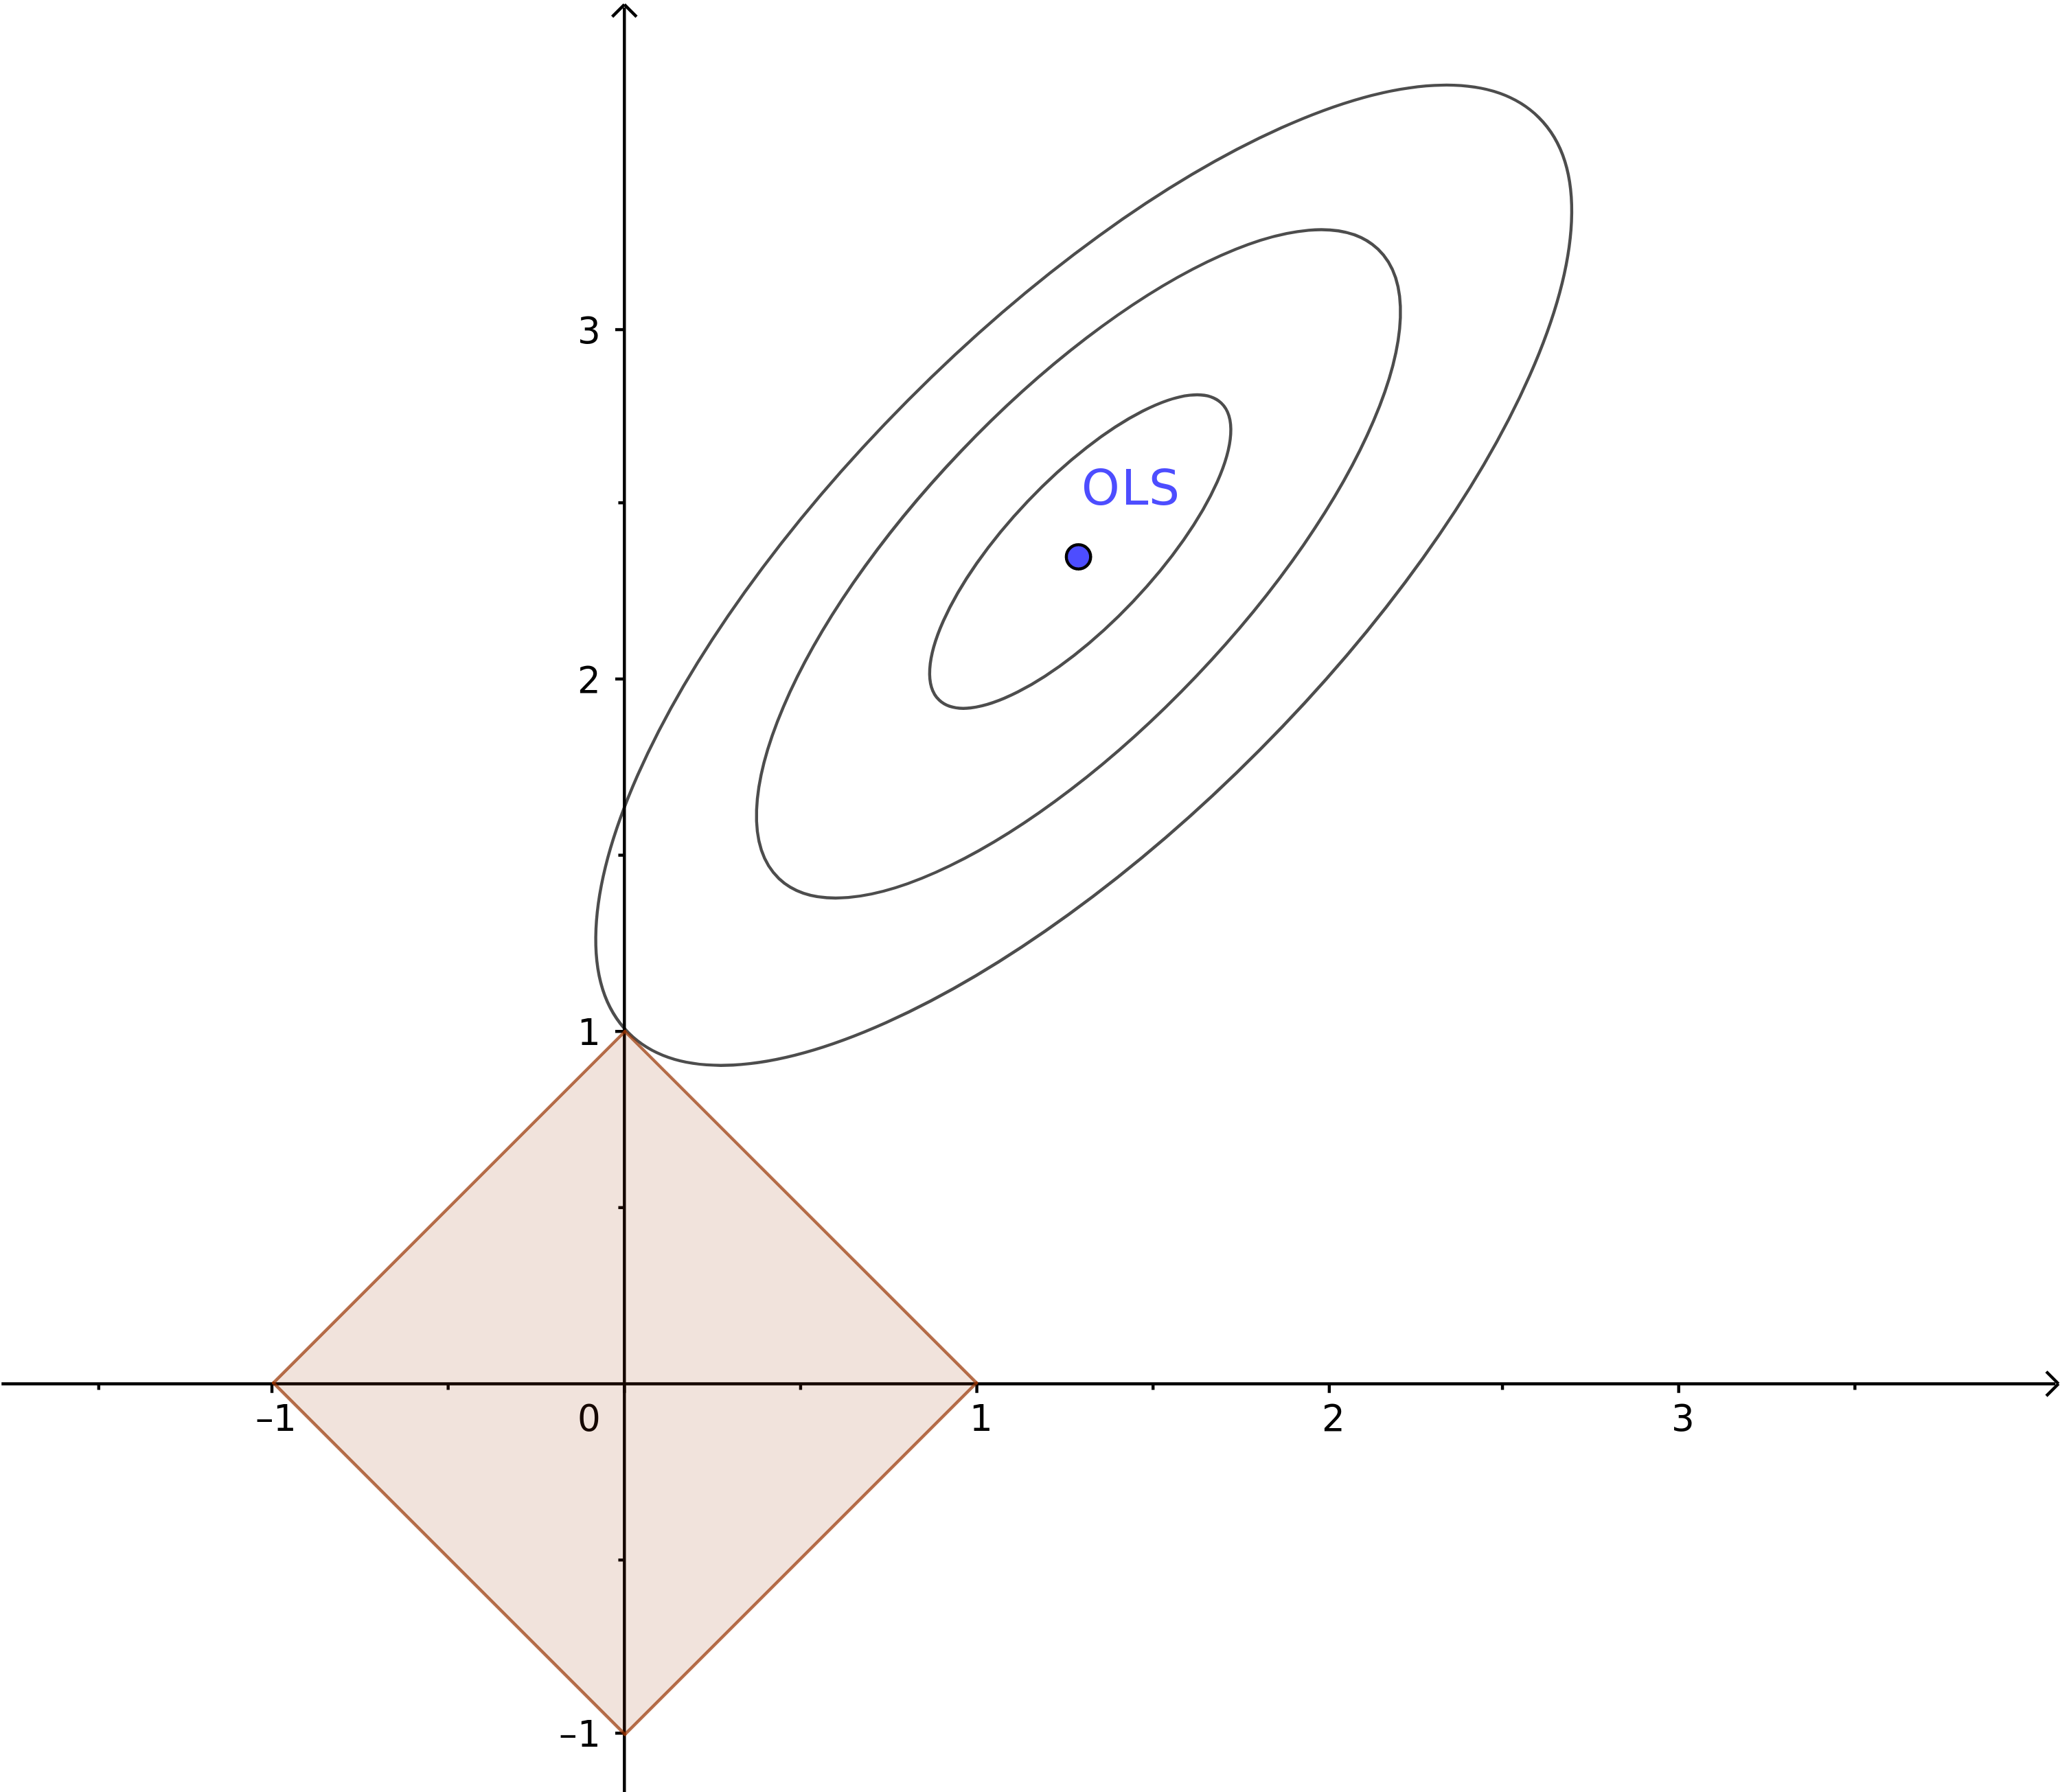
\includegraphics[width=\textwidth]{../../bld/out/figures/lasso_penalty.png}
	\caption{Lasso Penalty and OLS contour lines}
	\label{lassopenalty}
\end{figure}


%\begin{figure}[h!]
%	\centering
%	\includegraphics[width=0.5\textwidth]{../../out/figures/penalty.pdf}
%	\caption{Lasso penalty and contour lines of least squares, NOTIZ: müssen wir selber erstellen das Bild}
%	\label{lassopenalty}
%\end{figure}

\noindent\textbf{Drawbacks} \newline

\noindent If two variables are highly correlated Lasso tends to pick only one of them and which one sometimes depends on minor changes. \todo{Man könnte im Appendix ein Minimalbeispiel wie wir es in Computational hatten zur Veranschaulichung geben.} If both variables are supposed to be selected, the estimation can be done via the elastic net. The elastic net was developed to overcome the problem of lasso not identifying highly correlated covariates. It minimizes the objective function $\| Y-X\beta\|_2^2+\lambda_1 \| \beta\|_1 +\lambda_2\|\beta\|_2^2$. The additional penalty has the advantage that it makes the objective function strictly convex.

Lasso was designed for model selection and often has good predictive properties \citep{belloni2014}. However inference about model parameters such as regression coefficients has to be treated carefully. Lasso shrinks the coefficients of parameters and except for perfect model selecetion, can omit variables that have small influence in the model.

If there is information on the regressor structure, e.g. the $X_i's$ can be ordered in a meaningful way or there are regressors that can be seen as a group, we would like to include this information in the estimation. Examples can be found in time series, biology, image reconstruction and many more.
Lasso does not exploit the extra information when estimating. This gives rise to modifications of the Lasso, for example the fused lasso, which do so. 

\subsection{Solution methods}


%Lasso is a convec problem
The solutions to the minimization problem of the LASSO Estimator are the estimators $\hat\beta_\lambda$ that solve
$$\hat\beta_\lambda \in \argmin_{b\in \mathbb{R}^p}\underbrace{\frac{1}{n}\sum_{i=1}^{n}(y_i-x_i^Tb)^2+\lambda||b||_1}_{=S_\lambda (b)}.$$
%
Since the absolute value function is not differentiable at 0 we have to use subdifferential calculus, which is applicable because the objective is convex. In this simple case we can think of it as a widened interpretation of the derivative. The derivative of the absolute value function everywhere except at 0 is the sign function. So a quite natural idea is to say that the derivative of the function at 0 is characterized by the set $[-1,1]$. Calculating the left- and right-hand gradient leads to the Karush Kuhn Tucker conditions for this problem.

\begin{align*}
b_\lambda \in \argmin_{b \in\rm \mathbb{R}^p} S_\lambda(b) \Leftrightarrow \begin{dcases} 
\frac{1}{n}\sum_{i=1}^n x_{ij}(y_i-x_i'b)= \frac{1}{2}\lambda sgn(b_{\lambda,j}) &\ for \quad b_{\lambda,j} \neq0 \\   
\frac{1}{n}\sum_{i=1}^n x_{ij}(y_i-x_i'b) \leq  \frac{1}{2}\lambda \ &\ for \quad b_{\lambda,j}=0
\end{dcases} 
\end{align*}
This often leads to numerous components $\hat\beta_{\lambda,j}$ of the estimators dropping to 0 as described in Theorem \eqref{theo: sparsity_lasso}.

\todo{Brauchen eine Zitierung für die Subderivatives und Kuhn-Tucker Bedingungen.}

Since the optimization problem consists of sums of convex functions, computing the lasso estimator is in itself a convex optimization problem. That means we can use powerful algorithms to find the solution path. Also the lasso has the following useful property.\todo{An dieser Stelle sollten wir kurz und knapp den LARS Algorithmus erwähnen.}
\bigskip

\begin{theorem}(Convexity of solutions)\label{th: convexitylassosolution}
	Let $\hat{\beta}_{\lambda}$ and $\hat{\beta}_\mu$ be solutions of the minimization problem in (\ref{LassoLambda}) for $\lambda$ respectively $\mu$. Assume the two estimators have the same sign structure, then for any
	$\alpha\in[0,1]$ the linear combination $\alpha\hat{\beta}_{\lambda}+ (1-\alpha)\hat{\beta}_\mu$ is a solution to the minimization problem with penalty constant $\alpha \lambda + (1-\alpha) \mu$.
\end{theorem}

Convexity of the solution set can be helpful for calculating solution paths of the lasso. When one has calculated the lasso solution for two different penalty terms, where the estimators have the same sign structure, one does not need to solve the optimization problem for the penalties in between any more, but can simply use the formula for the estimator as in theorem \eqref{th: convexitylassosolution}.

\subsubsection{Coordinate descent} \label{Sec: Coordinate Lasso}
For fixed $\lambda_1$ the lasso estimator can be calculated by the coordinate descent algorithm.
Coordinate descent is an optimization method applicable in various contexts. It follows the idea that in some cases the minimization of a multivariate function can be conducted by successively solving univariate optimization problems for each variable. In a chronological order one minimizes over the current coordinate while fixing all other coordinates. For the lasso this means that we start for example with $\hat{\beta}_i =0$ for all $i$, then minimize over $\hat{\beta}_1$ while fixing the other coordinates, then minimize $\hat{\beta}_2$ fixing the other coordinates included the new estimate for $\hat{\beta}_1$. This procedure is done so long until the estimates barely change any more.
We can use coordinate descent because the objective function has the structure which is necessary for the algorithm to converge to the global minimum. The structure is
\begin{equation}
g(\beta_1,...,\beta_p)+\sum_{j=1}^Ph_j(\beta_j) \nonumber
\end{equation}
where $g: \mathbb{R}^p \to \mathbb{R}$, differentiable and convex and $h_j(\beta_j)$ are convex. Set $g(\beta_1,...,\beta_p)=\sum_{i=1}^{N}(y_{i}-x_{i}'\beta)^2$ and $h_j(\beta_j)=|\beta_j|$ for all j, then the above expression becomes the lasso objective function as in (\ref{LassoLambda}). Note that each $h_j(\beta_j)$ function only depends on one coefficient.
\cite[chapter 5]{sparsity}

\subsection{Lasso Signal Approximator}

To illustrate the material we first look at the special setting, where $X$ is the $n \times n$ identity matrix, thus $p=n$ and the regressors are orthonormal and thus in general position. The model then reduces to

$$Y_i=X \cdot\beta_i+\varepsilon_i=\sum^n_{j=1}I(j=i)\beta_i+\varepsilon_i = \beta_i + \varepsilon_i$$

We call the lasso estimator in this setting signal approximator as we can interpret $y$ as a signal with additive noise added and $\beta$ as the true signal.
Using the Karush Kuhn Tucker conditions we see that the unique lasso estimator in this case is
$$\hat\beta_{\lambda,j}= \begin{dcases} y_j-\frac{n\lambda}{2} &if \quad y_j>\frac{n\lambda}{2}\\
            									  y_j+\frac{n\lambda}{2} &if \quad y_j<-\frac{n\lambda}{2}\\
                                                  0						 &if \quad |y_j|\leq \frac{n\lambda}{2}
\end{dcases}$$
We can write this more compactly as 
\begin{equation}
 \hat\beta_{\lambda,j} = \sgn(y_j)(|y_j|-\frac{\lambda}{2})_+.
\end{equation}

\noindent In general we call $S_\lambda(z) := \sgn(z)(|z|-\frac{\lambda}{2})_+$ the soft-thresholding operator. In the orthonormal setting the lasso is thus the soft-thresholded OLS solution.
\todo{Könnten ein Bild einfügen.}
An interpretation of the solution is that only $\hat\beta_{\lambda,j}$ that contribute more than $\frac{n\lambda}{2}$ to explaining $y$ are unequal to zero. The coefficients that are unequal to zero are shrinked OLS estimates. The shrinkage is not proportional to the size of $y_j$, for all $y_j$ with $|y_j|\leq \frac{n\lambda}{2}$ the shrinkage of the absolute coefficient is by $\frac{n\lambda}{2}$.

\section{Fused Lasso}

\subsection{Definition and set-up}

Consider the same linear model setting as for the lasso with the following extension. Assume that there is a structure in $\beta$, such that neighboring $\beta_i$'s often have equal values. That means we have blocks of neighboring coefficients with the same values. We assume further that we only have a few, that means much less than $n$, blocks with nonzero coefficients. So the sparsity assumption of the lasso setting is relaxed.\\
Lasso does not use structural information within the features for the estimation. However this structure can be exploited by adding to lasso's objective function a second penalty term that penalizes differences between neighboring $\beta_i$'s, i.e. $\lambda_2\sum_{j=2}^p|\beta_j- \beta_{j-1}|$. This addition leads to the fused lasso estimator 
	\begin{equation}\label{eq: fusedlasso}
		\hat{\beta}_{\lambda_1,\lambda_2}^{FL}=\argmin_{\beta \in\rm \mathbb{R}^p} \left\{   \sum_{i=1}^{N}(y_{i}-x_{i}'\beta)^2+\lambda_1 \sum_{j=1}^p|\beta_j|+ \lambda_2 \sum_{j=2}^p|\beta_j- \beta_{j-1}| \right \}.
	\end{equation}
	
\todo{Es fehlt die analoge Schreibweise}

\subsection{The penalty constants} \label{subsec: penalties}
In contrast to the lasso case, we have two penalty constants. $\lambda_1$ is the coefficient on the lasso penalty and influences the estimator in the same way. $\lambda_2$ is the coefficient on the fusion penalty. \todo{Die penalties beeinflussen sich auch gegenseitig, müssen wir noch was zu schreiben.} For $\lambda_2=0$, we remain in the lasso problem. For an increasing $\lambda_2$, more and more neighboring $\beta_j$'s get 'fused' together, in the sense that $\beta_j=\beta_{j-1}$. For $\lambda_2\to\infty$, the objective function will be minimized at a vector $\beta$ that fulfills $\sum_{j=2}^p|\beta_j- \beta_{j-1}|=0$, so all coefficients get the same value.\\
As for the lasso, the penalty constants have to be chosen by the researcher.
Chosing the penalty constants incorporates prior information to the estimation. Harsh penalties only makes sense if one believes that the true $\beta$ vector is very sparse or the blocks where coefficients are equal are large. \\
A possible approach for chosing the penalty constants could be cross validation on a two dimensional grid. This can optionally be combined with a search strategy on the grid, for example a greedy strategy or meaningful starting points combined with fixed directions as proposed by \citep{fused}. Which method to use strongly depends on run time of the used algorithm as the problem can become computationally unfeasible. 
When considering grids an upper bound for $\lambda_1$ should be the optimal $\lambda$ of the lasso estimator.

\subsection{Properties of the solution}

Similar to the Lasso, we can define the following properties of the Fused Lasso estimator.

\begin{theorem}
	\begin{enumerate}
		\item[]
		\item \textbf{Existence} A solution of the minimization problem in (\ref{eq: fusedlasso}) always exists.
		\item \textbf{Uniqueness} \citep{ali2018generalized} Under 'non-redundancy' conditions on the design matrix $X$, the fused lasso estimator is unique.
	\end{enumerate}
\end{theorem}

\todo{Wir müssen schauen, ob man den Existenzbeweis von Lasso auf Fused Lasso verallgemeinern kann.}

\noindent\textbf{Advantages} \newline

\noindent Piecewise constant
\begin{theorem}[Sparsity of Fused Lasso] \citep{fused}
	Let $n_{seq}(\hat{\beta}) = \sum_{j=1}^{p} I \{\hat{\beta}_j \neq \hat{\beta}_{j-1}\}$ be the number of sequences of identical non-zero coefficients of the estimator. Then under 'non-redundancy' conditions on the design matrix $X$, we have $\hat{\beta}$ with $n_{seq}(\hat{\beta}) \leq N$.
\end{theorem}

\todo{Brauchen eine Interpretation der piecewise constant eigenschaft, averaging of the coefficients, außerdem müssen wir beschreiben wieso diese Eigenschaft wertvoll ist.}
\citet{rosset2007piecewise} give conditions under which the solution path of a regularized optimization problem is linear. They give conditions for a slightly different penalty term class but in chapter 5.2 they argue that the fused lasso is also piecewise constant.
\bigskip

\noindent\textbf{Drawbacks} \newline

The fused lasso estimator is not robust to model misspecifications, that means if it is applied to a setting, where we do not have a sparse block structure in the coefficients, it will not perform well.

The penalization is the same for all the coefficients no matter what the block length is. A smaller block needs a stronger penalization since it is more difficult to detect, a larger block needs less regularization. One way to overcome this problem is a modification of the fused lasso, namely the adaptive fused lasso (see \citep{rinaldoproperties}).


\subsection{Solution methods}

With the same argument as above for the lasso, computing the fused lasso estimator is a convex optimization problem. In contrast to the lasso problem the penalty term in the fused lasso problem is not separable in the single coefficients due to the second penalty. This makes the computation more complicated and coordinate descent is not an appropriate method any more as we will see now.

\subsubsection{Coordinate Descent}
In section \ref{Sec: Coordinate Lasso} we saw that the conditions for the coordinate descent to be a suitable solution method are fulfilled for the lasso. Unfortunately for the fused lasso this is not the case. The reason is that the separated non differentiable functions $h$ do not only depend on a single coefficient but on two. Take for example the fused signal approximator case, where we can set $\lambda_1 = 0$ (compare lemma \ref{sa: soft thresholding}). 
%Assume we have $p=100$ and coordinate descent sets the coefficients successfully to their optimal value. 
Assume that the previous iteration step set $\hat{\beta}_1=\hat{\beta}_2$ and we are in the new iteration step, where we minimize over $\beta_1$. Observe any change in $\beta_1$ introduces an increase of the absolute value of the difference of $\hat{\beta}_1$ and $\hat{\beta}_2$. Let us consider a situation in which it would be optimal to increase $\hat{\beta}_1$ a little to get rid of some squared differences in the model fit, but the difference in the absolute value is larger, so it is optimal for $\hat{\beta}_1$ to stay as in the previous iteration step. Assume we face the same problem in the iteration step for $\beta_2$, i.e. increasing it a little would be better for model fit, but it isn't done because of the combined penalty.
in such a scenario coordinate descent gets stuck. Therefore we have to use algorithms like gradient descent because they can move $\beta_1$ and $\beta_2$ simultaneously, so that here both increase slightly, so that the squared error gets smaller and the absolute difference stays 0.
A path algorithm is explained in the next section.
\cite[chapter 5]{sparsity}

%For the calculation of the solution one can make use of the following handy property of the fused lasso.
%
%
%\begin{lemma} \label{sa: behavior of optimum}[Behavior of the optimum] (cf. \citep{sparsity})
%	For any $\lambda_1' > \lambda_1$, we have
%	\begin{equation}
%		\hat{\beta_i}(\lambda_1', \lambda_2) = S_{\lambda_1'-\lambda_1} (\hat{\beta_i}(\lambda_1, \lambda_2)) \text{ for each } i = 1, \ldots, N,
%	\end{equation}
%	where $S$ is the soft-thresholding operator $S_\lambda(z) := \sgn(z)(|z|-\lambda)_+.$
%\end{lemma}
%\noindent	One important special case of Lemma \ref{sa: behavior of optimum} is the following equality, on which the path algorithm for the solution, which will be described in the next section, is based.

%\begin{equation}
%	\hat{\beta_i}(\lambda_1, \lambda_2) = S_{\lambda_1} (\hat{\beta_i}(0, \lambda_2)) \text{ for each } i = 1, \ldots, N.
%\end{equation}

\subsection{Fused Lasso Signal Approximator} \label{sec: fused_signal}

A special case of the fused lasso occurs when the predictor matrix is the $N \times N$ identity matrix. In this case the 'non-redundancy' conditions are fulfilled, so the estimator is unique. It has the following form.

	\begin{equation}
	\hat{\beta}_{\lambda_1,\lambda_2}^{FLSA}=\argmin_{\beta \in\rm \mathbb{R}^p} \left\{   \sum_{i=1}^{N}(y_{i}-\beta_i)^2+\lambda_1 \sum_{j=1}^p|\beta_j|+ \lambda_2 \sum_{j=2}^p|\beta_j- \beta_{j-1}| \right \}	
 \label{Fused-Signal}	\end{equation}

We can interpret the estimator as an approximator of an unknown signal which is blocky and sparse in its nature and corrupted by an additive noise. (cf. \citep{rinaldoproperties})

%\begin{lemma}[Soft thresholding property] \label{sa: soft thresholding} (cf. \cite{sparsity})
%	For any $\lambda_1' > \lambda_1$, we have
%		\begin{equation}
%		\hat{\beta_i}(\lambda_1', \lambda_2) = S_{\lambda_1'-\lambda_1} (\hat{\beta_i}(\lambda_1, \lambda_2)) \text{ for each } i = 1, \ldots, N,
%		\end{equation}
%	where $S$ is the soft-thresholding operator $S_\lambda(z) := \sgn(z)(|z|-\lambda)_+.$
%\end{lemma}

\begin{lemma}[Soft thresholding property] \label{sa: soft thresholding} (cf. \cite{sparsity})
	For any $\lambda_1 > 0$, we have
	
\begin{equation}
	\hat{\beta_i}(\lambda_1, \lambda_2) = S_{\lambda_1} (\hat{\beta_i}(0, \lambda_2)) \text{ for each } i = 1, \ldots, N.\footnote{Proofs of lemma \ref{monotone_fusion} and lemma \ref{sa: soft thresholding} can be found in the appendix.}
\end{equation}

\noindent where $S_\lambda$ is the soft-thresholding operator $S_\lambda(z) := \sgn(z)(|z|-\lambda)_+.$
\end{lemma}
	
The fused lasso is therefore a soft thresholded version of the fusion estimator. This fact can be exploited, when analyzing for example the asymptotics or writing algorithms for the solution.
\bigskip
	
Another useful property of the fused lasso estimator (only) in this easy setting is that of monotone fusion.

\begin{lemma}[Monotone Fusion] (cf. \citep{sparsity}) \label{monotone_fusion}
	Suppose that for some value of $\lambda$ and some index $i \in \{1, ..., -1 \}$ the optimal solution satisfies $\hat{\beta_i}(\lambda)$ = $\hat{\beta}_{i+1}(\lambda)$. Then for all $\lambda' > \lambda$, we also have $\hat{\beta_i}(\lambda')$ = $\hat{\beta}_{i+1}(\lambda')$.
\end{lemma}

\section{Asymptotics}

\label{sec:asymptoticslasso}

In this chapter we want to analyze asymptotics for the lasso and fused lasso. In general asymptotics for high dimensional statistical interference is difficult. The reason is that for a meaningful analysis, besides $n$ also $p$ needs to go to infinity and it even has to grow faster than $n$. Else at some point, $n$ would be bigger than $p$ and so we wouldn't be in a high dimensional setting any more. As soon as $p << n$, we can preferably use known methods as OLS since they do not come with a shrinkage bias.  
The problem, when analyzing the asymptotics with growing $p$ is that the underlying statistical model/DGP is changing as $p$ grows. Our usual central limit theorems do not hold any longer in this setting.
One way to handle high dimensional asymptotics is to work with triangular arrays. Roughly speaking a triangular array is a sequence with two indices, in which each row is only a long as the row's index.  For our linear model, this would be: $Y_{n;i}=\sum^{p_n}_{j=1}\beta^0_{n;j}X^{(j)}_{n;i}+\epsilon_{n;i}, \ i=1,...,n; \ n=1,2,...$.  \todo{Formel erklären} \newline

In this chapter we proceed as follows: We first briefly state some asymptotic results for the lasso, afterwards we speak about the asymptotics of the fused lasso signal approximator in more detail. The results in that section are valuable for the understanding of the fused lasso and the conditions under which it performs well. Finally we give an asymptotic normality result which includes the lasso as well as the fused lasso. The focus of the whole chapter is giving the interpretation and intuition of results as the scope of most of the proofs goes beyond this paper.

%An easy example of this is that of an urn. Consider an urn with 10 red and 10 blue balls. We would like to estimate the probability of drawing a red ball by repeatedly drawing from the urn (with replacing). In high dimensional settings, each time we draw from the urn, the distribution of red and blue balls changes inside the urn. In the following, we will give results on prediction error accuracy, convergence of the estimator and variable screening. 
%If we assume $||\beta^0||_1=||\beta_n^0||_1=o(\sqrt{\frac{n}{log(p)}}))$, $\epsilon$ as defined above and lambda in range of $\lambda=\lambda_n\asymp\sqrt{\frac{log(p)}{n}}$. The last assumption means that... . Then beta lasso is convergent in mean prediction sense. More formally $||X\hat{\beta}-X\beta^0||_2^2/n=o_P(1)$.
%If the covariates are not too correlated and on the sparsity assumption then if lambda is in the range of $\lambda=\lambda_n\asymp\sqrt{\frac{log(p)}{n}}$ then beta converges in probability to $\beta$: $||\hat{\beta}(\lambda)-\beta^0||_1=o_P(1)$. 
%We are interested if lasso is able to find the features with large coefficients. This is indeed the case as one can show that...

\subsection{Asymptotics Lasso} 

When considering the asymptotics of the lasso we are mainly interested in its selection property and its prediction accuracy.

Under no conditions on the design matrix and mild assumptions one obtains that
\begin{equation}
	||X\hat{\beta}-X\beta_0||_2^2/n \leq ||\beta_0||_1 O_p(\sqrt{(log(p)/n)}).
\end{equation}
This means that lasso is consistent in prediction if $\beta$ is sparse in the $\ell_1$-norm, more precisely $||\beta_0||_1 = o(\sqrt(n/log(p)))$.

In order to obtain optimal rates of convergence for prediction and estimation one needs to impose assumptions on the design matrix $X$. One imposes an eigenvalue or irerepresentability condition, which means....
\subsection{Asymptotics Fused Lasso Signal Approximator}

In this section we want to analyze asymptotic properties of the fused lasso signal approximator. The section follows closely \citep{rinaldoproperties}. Since $p = n$ is crucial for this setting as $n$ grows, $p$ needs to grow too.

As our main goal when applying the fused lasso is to do model selection our asymptotic analysis concentrates on two aspects: the conditions under which the block partition and the block sparsity pattern can be estimated correctly. By block partition we mean the partition $\{B_1, \ldots, B_{J_0}\}$ of $\{1, \ldots, n\}$ into sets of consecutive indexes, such that we can write the coefficient vector $\beta$ as
\begin{equation}\label{eq: beta_fused_signal}
	\beta = \sum_{j=1}^{J_0} v_j I(j \in B_j).
\end{equation}
The block sparsity pattern is the set $JS(\beta) = \{j: v_j \neq 0\}$, i.e. the indexes of the nonzero blocks. We will see that the conditions consist of conditions on the sequences of regularization parameters $\lambda_{1,n}$ and $\lambda_{2,n}$ and on the structure and values of the coefficient vector $\beta$.
We begin by defining assumption (E): \\

\noindent (E) The errors $\varepsilon_i, 1 \leq i \leq n$ are all identically distributed centered Gaussian variables with variance $\sigma_n^2$ such that $\sigma_n \to 0$. \newline

\noindent An example for such a variance would for example be $\sigma_n = \sigma /n$ 


\begin{theorem}
	Assume (E) and a structure of $\beta$ as in \eqref{eq: beta_fused_signal}. If the conditions on $\lambda_{1,n}$ and $\lambda_{2,n}$, on the minimal size of blocks, the smallest amplitude of blocks and the smallest difference between blocks as spelled out in \citep{rinaldoproperties} are fulfilled then for the set
	\begin{equation}
		R_{1,n} = \{JS_0 = \hat{JS}\} \cap \{\forall j\in JS_0: \sgn(v_j) = \sgn(\hat{v}_j)\}
	\end{equation} 
	
	\noindent we have $\lim_n P(R_{1,n}) = 1$.
\end{theorem}
This result is obtained as follows: First one derives the conditions under which the fusion estimate consistently recovers the true block partition and the local maxima and minima of $\beta$. Here consistency demands 

\begin{enumerate}
	\item The penalty constant $\lambda_{2,n}$ needs to increase with a specific rate.
	\item The magnitude of the smallest jump (distance between two blocks) does not vanish faster than a specific rate. This means the blocks can asymptotically be distinguished. Also the smallest block (by number of indexes) must not be too small. The larger the size of a block, the easier is its recovery by the estimator.
	\item The penalty constant needs to be smaller than a specific value, which incorporates the smallest jump and smallest block. If the smallest block or jump is small, $\lambda_{2,n}$ must not be too large in order not to fuse blocks that are not fused in $\beta$. 
\end{enumerate} 
 
In section \eqref{sec: fused_signal} we have seen that the fused lasso signal approximator is the soft-thresholded fusion estimate. Thus one knows that under the conditions for consistently estimating the blocks and extrema for the fusion estimate also the fused lasso consistently recovers them. This is due to soft thresholding not changing the block partition. Next one wants to know under which additional conditions not only the true local minima and maxima can be detected, but also the true block sparsity pattern can be achieved. We can qualitatively summarize the conditions as:
\begin{enumerate}
	\item The penalty constant $\lambda_{1,n}$ needs to increase with a specific rate.
	\item The magnitude of the smallest nonzero block value cannot decrease to zero too fast. This guarantees some asymptotic distinguishability between zero and non-zero blocks.
	\item Since the two penalty constants influence each other (see section \eqref{subsec: penalties}) they need to be in a certain ratio for each $n$ to enable the detection of the true blocks.
\end{enumerate}

\subsection{Asymptotic Normality}
In the following we cite an asymptotic result from \citet{fused} and give an interpretation hereof.
For simplicity the authors assumed that $p$ is fixed with $N \rightarrow \infty$. As the authors note themselves these are ``not particularly realistic asymptotic conditions'' as the lasso and fused lasso are methods for high-dimensional data, which is not the case any more if $N$ gets larger than $p$. Still we think that the interpretation of the result is insightful.

\begin{theorem} (\citep{asymptoticslasso},\citep{fused}) \newline
	If $\lambda_N^{(l)}/\sqrt{N} \rightarrow \lambda_0^{(l)} \geq 0 \  (l=1,2)$ and
	\begin{equation*}
	C = \lim\limits_{N \rightarrow \infty}{(\frac{1}{N} \sum_{i=1}^{N}x_i x_i^T)}
	\end{equation*}
	is non-singular then
	\begin{equation*}
	\sqrt{N}(\hat{\beta}_N - \beta) \rightarrow_{\text{d}} \argmin(V),
	\end{equation*}
	where
	\begin{align*}
	V(u) = &-2u^T W + u^T Cu + \lambda_0^{(1)} \sum_{j=1}^{p} \{u_j \sgn(\beta_j)I(\beta_j \neq 0) + |u_j|\ I(\beta_j=0) \} \\
	&+ \lambda_0^{(2)} \sum_{j=2}^{p} \{(u_j - u_{j-1}) \sgn(\beta_j - \beta_{j-1})I(\beta_j \neq \beta_{j-1}) + |u_j-u_{j-1}|\ I(\beta_j=\beta_{j-1}) \}, 
	\end{align*}
	with $u \in \mathbb{R}^p$ and $W$ has an $\mathcal{N}(0,\sigma^2 C)$ distribution.
\end{theorem}

The idea of the theorem and proof is similar to that in \citep{asymptoticslasso} where the asymptotics of the Lasso are analyzed. In order to study the limiting behavior of the fused lasso the asymptotic behavior of a specific objective function is studied. This objective function is minimized at $\sqrt{N}(\hat{\beta}_n-\beta)$ and converges in distribution to $V(u)$. The proof of the theorem can be found in \citep{fused}, we will give an interpretation of the result.\newline

\noindent We first look at the sequence of regularization parameters $\lambda_N^{(l)}$, where $l=1,2$. The expression $\lambda_N^{(l)}/\sqrt{N} \rightarrow \lambda_0^{(l)} \geq 0$ means that as $n$ grows to infinity, the penalty constants need to be modified. They need to grow in a particular speed, namely $\lambda_N^{(l)}$ are $o(\sqrt{N})$. The reason is that for growing $N$ there is a chance of overfitting if $\lambda$ stayed constant, the estimator would pick up irrelevant regressors if the penalization is not harsh enough.\newline

When taking a closer look at the function $V(u)$, we notice that only the first part of the function containing $W$ is stochastic. The second part can be seen as a bias term as we will describe now further. \newline

We start with the case, where $\lambda_0^{(1)}= \lambda_0^{(2)} = 0$, so we are back to the OLS setting. The function $V(u)$ reduces to $V(u) = -2u'W + u'Cu$. It is easy to see that this is minimized at $C^{-1}W$, so as expected 		$\sqrt{N}(\hat{\beta}_N - \beta) \rightarrow_{\text{d}} \mathcal{N}(0,\sigma^2 C^{\frac{1}{2}})$.
When $\lambda_0^{(1)}$ and/or $\lambda_0^{(2)}$ are unequal to zero we will not get asymptotic normality centered at zero as we will see now. \newline

We want to interpret the results for $\lambda_0^{(1)}, \lambda_0^{(2)} > 0$ by means of an example. Therefore we consider the case where $\beta \in \mathbb{R}^2$.
%Tibshirani et al. define $V_N(u)$ by
%\begin{align*}
%	V_N(u)= &\sum_{i=1}^{N} \{(\varepsilon_i - u^Tx_i/\sqrt{N})^2 -\varepsilon_i^2 \} + \lambda_N^{(1)} \sum_{j=1}^{p}(|\beta_j + u_j / \sqrt{N}|-|\beta_j|) \\
%	&+ \lambda_N^{(2)} \sum_{j=2}^{p} \{ |\beta_j - \beta_{j-1}+(u_j-u_{j-1})/\sqrt{N}|-|\beta_j - \beta_{j-1}|\}.
%\end{align*}
%
%The design of $V_N(u)$ is such that it is minimized at $\sqrt{N}(\hat{\beta_n}-\beta) $. \todo{Could prove this}
%Furthermore they show that $V_N(u) \rightarrow_{\text{d}} V(u)$ with finite-dimensional convergence holding as well \citep{fused}.
%They conclude that since $V_N$ is convex and $V$ has a unique minimum, it follows that \todo{Need an explanation of this fact since the reference paper is not online}
%\begin{equation*}
%	\argmin(V_N) = \sqrt{N}(\hat{\beta_N}-\beta) \rightarrow_{\text{d}} \argmin(V).
%\end{equation*}

We start by taking the (sub)derivative of $V$ with respect to $u_1$ and setting it to zero.

\begin{align} \label{eq: subder}
	0 = -2w_1 + 2c_{11}u_1 + u_2 (c_{12}+c_{21}) &+ \lambda_0^{(1)}(\sgn(\beta_1) I(\beta_1 \neq 0) + \sgn(u_1)) \nonumber\\
	 &+ \lambda_0^{(2)} (-\sgn(\beta_2-\beta_1))I(\beta_1 \neq \beta_2) \nonumber\\
	 & \quad \quad \quad - \sgn(u_2-u_1)I(\beta_2 \neq \beta_1)) 
\end{align}

\noindent By $\sgn(z)$ we denote the subderivate of the absolute value of $z$. It corresponds to the derivative of the absolute value, the sign function, whenever $z \neq 0$ and to the set $[-1,1]$, when $z=0$.\\

The first case we want to look at is $\lambda_0^{(1)} > 0$ and $\lambda_0^{(2)} = 0$, so we are in the lasso setting. If $\beta_1 \neq 0$ we can derive a closed form solution for $\argmin(V)$.

\begin{equation}
	u_1 = \frac{1}{2c_{11}} (2w_1 - u_2(c_{12}+c_{21})-\lambda_0^{(1)} \sgn(\beta_1))
\end{equation}

\noindent The first two summands correspond to the minimum in the OLS case, so we see that the penalty term introduces a bias. We know that lasso does shrinkage of the absolute value of the parameters, so for $\beta$ positive, $\hat{\beta}$ will be smaller and for $\beta$ negative $\hat{\beta}$ will be larger than in the OLS setting. This is also true asymptotically. Therefore with growing $n$ the scaled difference $\sqrt{n}\hat{\beta} - \beta$ has a shift of probability to the negative side if $\beta$ is positive and a shift of probability to the positive side if $\beta$ is negative.\\

Now we consider the case where $\lambda_0^{(1)} = 0$ and $\lambda_0^{(2)} > 0$, so we are in the fusion setting. For $\beta_1 \neq \beta_2$ we can derive the following closed-form solution for $u_1$.

\begin{equation}
u_1 = \frac{1}{2c_{11}} (2w_1 - u_2(c_{12}+c_{21})+\lambda_0^{(2)} (\sgn(\beta_2)-\sgn(\beta_1))
\end{equation}

\noindent Again the first two summands correspond to the minimum in the OLS case, so also $\lambda_0^{(2)}$ introduces a bias asymptotically. The fusion estimator will try to fuse the coefficients together or reduce the distance between them. Therefore if $\beta_2 > \beta_1$, the estimate $\hat{\beta}_1$ will be larger than in the OLS setting. Thus with growing $n$ the scaled difference $\sqrt{n}\hat{\beta} - \beta$ has a shift of probability to the positive side. Vice versa when $\beta_1 > \beta_2$.

If we now consider $\lambda_0^{(1)} > 0$ and $\lambda_0^{(2)} > 0$ we can see from the above considerations that only in some cases the direction of the asymptotic bias is clear. For example if $\beta_1 > 0$ and $\beta_2 > \beta_1$ there is a positive shift of probability, if $\beta_1 > 0$ and $\beta_2 < \beta_1$ the direction of the bias is though not clear.

Note that from equation \eqref{eq: subder} one can also see that when some of the $\beta_j$s are exactly $0$, the limiting distributions put positive probability at $0$ and when $\beta_1 = \beta_2$ probability is centered at the line $u_1 = u_2$. 


\newpage

\section{Simulation}

To provide some comparison between lasso and fused lasso, we performed simulations with both methods on different settings. The data for each simulation setting were generated with $p=500$ and $N=50$. In all simulations we used the same fixed design matrix $X\sim \mathcal{N}(0,\mathcal{I})$. We vary the coefficient structure of the features $\beta$ and $\varepsilon$ in each simulation step to incorporate differently arranged $\beta$. In each simulation setting we chose the structure of the features generation process such that we incorporate relevant cases.\\

For the four following simulation settings the number of relevant features was set to 30. This was done to show differences in performance depending rather on the structure than on the number of relevant features.\\
The first setting was constructed as the basic example, where fused lasso might have advantages over lasso. We only include one block of relevant features of length 30. In the second setting we split the relevant features into 3 equally long blocks, that might or might not be neighboring each other. This provides us an intuition on how the estimation of $\beta$ with fused lasso might depend on the amount of blocks into which the relevant features are split. In the third setting we extend the setting by allowing the blocks in $\beta$ to have different height. In the fourth setting, we augment the number of relevant features by adding a small number of spikes into $\beta$, in the area of non relevant $\beta_j$. This illustrates a case where fused lasso might have problems, picking up the solitary relevant features.\\

To perform lasso or fused lasso on this simulation setting, we need to provide the penalty constants $\lambda_1,\lambda_2$ or the equivalent constraint boundaries $s_1, s_2$. As described in subsection \ref{subsec: penalties} there are different methods to calculate the two penalty constants. Since we are able to do cross-validation over a whole two-dimensional grid in a reasonable time, we decided not to use a search strategy. The proposed direction for the search pattern in \citet{fused} was only justified by “empirical experimentation", which was not further explained and therefore might not be adequate for our setting. By optimizing over the whole grid we make sure to not miss the optimal combination of $\lambda_1$ and $\lambda_2$.\\

Since we build our fused lasso estimator as an extension of the ``BaseEstimator'' of Sklearn \citep{scikit-learn}, we can resort to the build in ``GridCV'' to perform k-Fold cross-validation over a grid of hyperparameters $s_1,s_2$. We chose to perform 3-fold cross-validation. That means our sample was divided into three folds, of whom always two were used to fit our model and perform a prediction on the remaining fold. The ``prediction'' fold was permutated until all folds were once used as prediction fold.\\
To evaluate which $s_1,s_2$ pair was to be preferred in this setting, we relied on the mean prediction error.
\\


We implemented the fused lasso estimator with the cvxpy package for convex optimization problems \citep{cvxpy}\footnote{Correctness of the package was checked by our own computations and algorithms of the estimators.}. The package enables a fast calculation of the estimators even for reasonably large $p$ and $n$. \\

One of the main goals of our estimators is model selection. That means in order to analyze how well the estimators perform on our simulated data we need to analyze their so called specificity and sensitivity. Specificity means the proportion of the true zero coefficients and sensitivity the proportion of the true non-zero coefficients that are detected by the estimated model.



Possible structures of coefficients for the simulation:
\begin{enumerate}
	\item plateaus (of different size) already implemented
	\item plateaus and one(ore more) peaks
	\item sparsity, but without plateaus
	\item situations in which the lasso or fused lasso may not be appropriate (imposing a wrong prior):
	\begin{enumerate}
		\item no ordering of the features
		\item no sparsity
	\end{enumerate}
\end{enumerate}

\todo{Insert images from simulation and evaluation. Müssen package booktabs benutzen.}



\section{Real Data Application}

\subsection{Comparative Genomic Hybridization Data}
The first application we want to consider is from medical science. We want to look at data from Comparative Genomic Hybridization (CGH), a powerful method for molecular analysis of cancer.    
CGH provides an overview of changes in DNA sequence copy number in a tumor sample 
%and maps these changes on normal chrosomosomes
relative to a control sample, i.e. normal chromosomes. Changes can be in form of losses, deletions, gains and amplifications\citep{cghmain}. The DNA  sequence copy number is then given as a function of chromosomal location throughout the entire genome, the genetic material of an organism \citep{cghsecond}. This can for example look as in figure (\ref{cghdata}).

\begin{figure}
	\centering
	\includegraphics[width=\textwidth]{../../bld/out/figures/cgh_plot.pdf}
	\caption{CGH Data}
	\label{cghdata}
\end{figure}

The CGH data are coming from an experiment and are very noisy. This renders some kind of smoothing necessary before analysing the data. \\
Biological considerations dictate that it is typically segments of a chromosome — rather than individual genes — that are replicated, Consequently, we might expect that the underlying vector of true copy numbers to be piecewise-constant over contiguous regions of a chromosome.
In this specific example we have as many regressors (genes) as observations (copy numbers) \citep{sparsity}.
As seen above the fused lasso signal approximator is designed for cases like these with $ p = n$ and a meaningful ordering of the coefficients

\section{Conclusion/Discussion}

Have looked at specific penalized regression.

\begin{enumerate}
	\item Neighbors generalize to neighboring areas  (for example image reconstruction for 2d case, cf. \citep{sparsity})
	\item Several different choices for the penalties on neighboring coefficients (apart from the $\ell^1$-norm) are possible.
	\item Assume a uniformly spaced index, can consider cases where the index variable has nonuniform values (see p.667 in \citep{sparsity})
	\item Can consider case where the features are unordered.
	\item generalizations on the penalties and on the model fit possible
\end{enumerate}
 %\citep{adams1995hitchhiker}
 
 \citep{elements}

\appendix

\newpage

\section{Code}




%beispiel für manuelle eingabe
%\lstset{title={Titile}}
%\begin{python}
%import numpy as np%
%
%log_of_two = np.log(2)

%string = 'hello world'

%def square(x)

%	return x**2
	
%class MyClass():
%\end{python}

%so ist es wohl am einfachsten
\lstset{title={flestimator.py}}
\pythonexternal{../../src/model_code/flestimator.py}

\todo{Insert code for simulation with lasso and fused lasso as soon as the question is being answered how to optimize over both lambdas}


\section{Proofs}

\subsection{}Equivalence of (\ref{Primal}) and (\ref{LassoLambda}):
First of all note that for any $b$ with $||b||_1 > \frac{||Y||^2}{\lambda}$ the following inequality holds:
\begin{equation}
	S_\lambda(b) \geq \lambda ||b||_1 > ||Y||^2 = S_\lambda(0).
\end{equation}

that means the Lasso criterion is smaller for $\tilde{b}=0$, so $b$ is not a solution.
Thus we have
\begin{equation*}
 \hat{\beta}_\lambda^{Lasso} = \argmin_{\beta \in\rm \mathbb{R}^p} S_\lambda(b) = \argmin_{\substack{\beta \in\rm \mathbb{R}^p\\ ||b||_1 \leq \frac{||Y||^2}{\lambda}}} S_\lambda(b)
\end{equation*}
so the two ways of writing the estimator are equivalent.

\subsection{}\begin{proof} Convexity of solution set for fixed $\lambda$ \newline
Define the objective function
\begin{align*}
h(\beta)=\|Y-X\beta\|_2^2+\lambda\|\beta\|
\end{align*}
Note that $h(\beta)$ is convex. Let $\beta_1$ and $\beta_2$ be two minimizers of $h(\beta)$ and let $\beta_3=\alpha\beta_1+(1-\alpha)\beta_2$ where $\alpha \in (0,1)$. Then due to convexity of $h(\beta)$ for any $\beta \in \mathbb{R}^p$ we have
\begin{align*}
h(\beta_3)&=h(\alpha\beta_1+(1-\alpha)\beta_2) \leq \alpha \underbrace{h(\beta_1)}_{\leq h(\beta)}+(1-\alpha)\underbrace{h(\beta_2)}_{\leq h(\beta)} \\ &\leq \alpha h(\beta)+(1-\alpha)h(\beta)=h(\beta) \\ &\Rightarrow \alpha\beta_1+(1-\alpha)\beta_2 \ \ \ \text{is also a minimizer}
\end{align*}
Note that this implies that in case Lasso has two solutions there are uncountably many solutions.
\end{proof}

\subsection{} \begin{proof} Existence \newline
Consider the problem written as in (\ref{Primal}). Observe that the arg min is taken over a compact set and the squared $\ell^2$ norm is a continuous function. By the extreme value theorem it follows that there always exists at least one solution to the minimization problem.
\end{proof}

\subsection{}

\todo{Ich finde die Notation in dem Beweis nicht gelungen, für Fused Lasso hatten wir die Lambdas bisher unten und nicht oben.}
\begin{proof} Lemma \ref{sa: soft thresholding} (The basis of this proof can be found in \citep{friedman2007pathwise})
	We want  to show that the solution to this problem 
	\begin{equation}
	\frac{1}{2}  \sum_{i=1}^{6}(y_{i}-\beta_i)^2+\lambda_1\sum_{i=1}^p|\beta_i| + \lambda_2 \sum_{j=2}^6|\beta_j- \beta_{j-1} |
	\end{equation} is equivalent to first calculate the solution for some lambda2  and $\lambda_1 =0$ and then soft thresholding it with $\lambda_1>0$. We argue as follows: the soft thresholded estimator also solves the gradient equation which is necessary and sufficient for it to be a solution. The gradient function for some $\beta_j$ is given by
	\begin{equation}
	-(y_j-\hat{\beta}_j)+\lambda_1 sgn(\beta_j)+\lambda_2 [sgn(\hat{\beta}_j-\hat{\beta}_{j-1})+sgn(\hat{\beta}_{j+1}-\hat{\beta_j})]=0
	\end{equation}
	Assume we calculated a solution for $\lambda_1=0$ and $\lambda_2 > 0$ denoted by $\hat{\beta^0}$. The soft thresholded version of it is given by $\hat{\beta^{\lambda_1}}=sgn(\hat{\beta^0})(|\hat{\beta^0}|-\lambda_1)^{\text{+}}$. The next step is that we plug it into the above equation and argue that it holds. Before we note some observations. Note that if $\hat{\beta}^0_j=0$ then we are free to choose $sgn(\hat{\beta}^0_j) \in [-1,1]$, for convenience we set it to 0. Next we compare the differences $sgn(\hat{\beta}_j^0-\hat{\beta}_{j-1}^0)$ with $sgn(\hat{\beta}_j^{\lambda_1}-\hat{\beta}_{j-1}^{\lambda_1})$. There are two cases: if after the thresholding one parameter is set to 0 and the other one unequal to zero we know that betas just changes in the level so the differences stays the same, the other case is if both get shrunken to zero, then since $sgn(0)$ we are free to choose the value, especially we can set equal to the non thresholded estimators. So it follows $sgn(\hat{\beta}_j^0-\hat{\beta}_{j-1}^0)=sgn(\hat{\beta}_j^{\lambda_1}-\hat{\beta}_{j-1}^{\lambda_1})$. Finally we can plug the soft thresholded estimator in the derivative condition.
	\begin{align}
	-y_j+sgn(\hat{\beta}^0_j)(|\hat{\beta}_j^0|-\lambda_1)^{\text{+}}+\lambda_1 sgn(\hat{\beta}_j^{\lambda_1})+\lambda_2 [sgn(\hat{\beta}^{\lambda_1}_j-\hat{\beta}^{\lambda_1}_{j-1})+sgn(\hat{\beta}^{\lambda_1}_{j+1}-\hat{\beta}^{\lambda_1}_j)]=0
	\end{align}
	Consider the case  where $|\hat{\beta^0}|-\lambda_1\geq0$, noting the equality $sgn(\beta)|\beta|=\beta$ and the fact that the sign of the differences is the same as for lambda equal to we are left with
	\begin{equation}
	-y_j+\hat{\beta}_j^0-\lambda_1 sgn(\hat{\beta}^0_j) + \lambda_1sgn(\hat{\beta}^{\lambda_1}_j)+\lambda_2 [sgn(\hat{\beta}^{0}_j-\hat{\beta}^{0}_{j-1})+sgn(\hat{\beta}^{0}_{j+1}-\hat{\beta}^{0}_j)]=0
	\end{equation}
	So by setting $sgn(\hat{\beta}^0_j)=sgn(\hat{\beta}^{\lambda_1}_j)$ equation 20 reduces to the optimality condition if lambda1 is equal to 0 and since we assumed $\hat{\beta}^0$ is the solution for this problem we know the equation holds.
	In case two if $|\hat{\beta}_j^0|-\lambda_1<0$ then $\hat{\beta}_j^{\lambda_1}=sgn(\hat{\beta}_j^0)(|\hat{\beta}_j^0|-\lambda_1)^{\text{+}}=0$. Ignoring by the same arguments the sign differences we are left with
	\begin{equation}
	-y_j+\lambda_1 sgn(\hat{\beta}_j^{\lambda_1})
	\end{equation}
	Since we can chose the sign to be anywhere between -1 and 1 we set it to $\frac{\hat{\beta}_j^{0}}{\lambda_1}$
\end{proof}

\subsection{}
\begin{proof} Idea: Monotone Fusion Property \citep{friedman2007pathwise}
For simplicity we assume soft thresholding property is true. That means we can set $\lambda_1=0$ and we have n=p=6. Then the objective function looks as follows
\begin{equation}
\frac{1}{2}  \sum_{i=1}^{6}(y_{i}-\beta_i)^2+ \lambda_2 \sum_{j=2}^6|\beta_j- \beta_{j-1} |
\end{equation}
Let's assume we know the solution and it satisfies $\hat{\beta}_3=\hat{\beta}_4=\hat{\beta}_5=\hat{\beta}^*$ and $\hat{\beta}_2\neq\hat{\beta}^*$ and $\hat{\beta}_6\neq\hat{\beta}^*$ It follows that $sgn(\hat{\beta}_3-\hat{\beta}_2)$ and $sgn(\hat{\beta}_6-\hat{\beta}_5)$ are both $\in \{-1,1\}$ further $sgn(\hat{\beta}_4-\hat{\beta}_3)$ and $sgn(\hat{\beta}_5-\hat{\beta}_4)$ vary in $[-1,1]$. The partial derivative's of the objective function evaluated at the solution are given by
\begin{align}
-(y_1-\hat{\beta}_1)+\lambda_2 sgn(\hat{\beta}_2-\hat{\beta_1})=0 \\
-(y_2-\hat{\beta}_2)+\lambda_2 [sgn(\hat{\beta}_2-\hat{\beta_1})+sgn(\hat{\beta}_3-\hat{\beta_2}))]=0 \\
-(y_3-\hat{\beta}_3)+\lambda_2 [\underbrace{sgn(\hat{\beta}_3-\hat{\beta_2}}_{Boundary})+sgn(\hat{\beta}_4-\hat{\beta_3})]=0 \\
-(y_4-\hat{\beta}_4)+\lambda_2 [sgn(\hat{\beta}_4-\hat{\beta_3})+sgn(\hat{\beta}_5-\hat{\beta_4})]=0 \\
-(y_5-\hat{\beta}_5)+\lambda_2 [sgn(\hat{\beta}_5-\hat{\beta_4})+\underbrace{sgn(\hat{\beta}_6-\hat{\beta_5})}_{Boundary}]=0 \\
-(y_6-\hat{\beta}_6)+\lambda_2 [sgn(\hat{\beta}_6-\hat{\beta_5})+sgn(\hat{\beta}_7-\hat{\beta_6})]=0 
\end{align}
Since the sgn functions which evaluate exactly to -1 or 1 are fixed ,they can be seen as boundaries for the "inner" differences. And so the inner differences only depend on  a sub system of the above equations. The differences $(12)-(11)$ and $(11)-(10)$ can be written as. 
\begin{align}
\left(\begin{matrix}2&-1\\-1&2\end{matrix}\right)\left(\begin{matrix}sgn(\hat{\beta}_4-\hat{\beta_3})\\sgn(\hat{\beta}_5-\hat{\beta_4})\end{matrix}\right)&=\frac{1}{\lambda_2} \left(\begin{matrix}y_4-y_3\\y_5-y_4\end{matrix}\right) + \left(\begin{matrix}sgn(\hat{\beta}_3-\hat{\beta_2})\\sgn(\hat{\beta}_6-\hat{\beta_5})\end{matrix}\right) \\ \Rightarrow \left(\begin{matrix}sgn(\hat{\beta}_4-\hat{\beta_3})\\sgn(\hat{\beta}_5-\hat{\beta_4})\end{matrix}\right)&=\frac{1}{\lambda_2} \left(\begin{matrix}\frac{1}{2}&\frac{1}{4}\\\frac{1}{4}&\frac{1}{2}\end{matrix}\right)   \left(\begin{matrix}y_4-y_3\\y_5-y_4\end{matrix}\right) \\ &+  \left(\begin{matrix}\frac{1}{2}&\frac{1}{4}\\\frac{1}{4}&\frac{1}{2}\end{matrix}\right)      
  \left(\begin{matrix}sgn(\hat{\beta}_3-\hat{\beta_2})\\sgn(\hat{\beta}_6-\hat{\beta_5})\end{matrix}\right)
\end{align}
Note that both entries in (16) are always between -1 and 1. We also know that the sgn function in (15) are between -1 and 1. If $\lambda:2$ increases it only shrinks the values closer to 0. Thus we see $\hat{\beta}^*$ might change but that fused set remains constant. Since the structure of the solution remains intact. Only if a new beta joins the group say beta2, but then we could repeat the same argument.
\end{proof}

\newpage
\bibliography{refs}

\end{document}

%
%\section{Lasso}
%    \subsection{Characterization of the LASSO-Solution}
%    For the Lasso criterion  
%    $$ \min_{b\in\RR^p}S_\lambda(b)=\frac{1}{n}(y_i-X_i^Tb)^2+\lambda||b||_1,\qquad \lambda>0$$
%    there exists $ b_\lambda\in\argmin_{b\in R^p}S_\lambda(b)$.\footnote{Proof: For }

